% Bone fracture detection: CNN vs ScatNet + XAI -- 12-minute exam presentation.
% Build: make (or: latexmk -pdf main.tex). Numbers, tables and figures come from ../results/
% (written by the notebook); missing ones show a grey placeholder, so the slides always compile.
\documentclass[aspectratio=169,10pt]{beamer}
\usetheme[progressbar=frametitle,numbering=fraction,sectionpage=none]{metropolis}
\usepackage[T1]{fontenc}
\usepackage[sfdefault,scaled=.9]{FiraSans}
\usepackage{booktabs,amsmath,amssymb,graphicx,etoolbox,xcolor}
\usepackage{tikz}
\usetikzlibrary{positioning,arrows.meta,fit,calc,shapes.misc}

\providecommand{\resultsdir}{../results}
\IfFileExists{\resultsdir/latex/numbers.tex}{\input{\resultsdir/latex/numbers.tex}}{}
% Fallback values: every macro written by src/report.py (results/latex/numbers.tex).
% \providecommand only defines a macro that the results did not define, so after a run
% the real numbers win and before a run the slides still compile, showing "--".
\newcommand{\na}{\textcolor{gray}{--}}
\providecommand{\BestModel}{\na}
\providecommand{\BestModelKey}{none}
\providecommand{\SelectBy}{F1}
\providecommand{\Epochs}{20}
\providecommand{\KFolds}{5}
\providecommand{\NTrain}{9{,}246}
\providecommand{\NVal}{829}
\providecommand{\NTest}{506}
\providecommand{\DupTrain}{\na}
\providecommand{\DupTrainPct}{\na}
\providecommand{\DupGroups}{\na}
\providecommand{\DupVal}{\na}
\providecommand{\DupValPct}{\na}
\providecommand{\DupTest}{\na}
\providecommand{\DupTestPct}{\na}
\providecommand{\ScratchMaxDiff}{\na}
\providecommand{\McNemarCNNvsScat}{\na}
\providecommand{\McNemarCNNvsRes}{\na}
\providecommand{\McNemarScatvsRes}{\na}
\providecommand{\ScratchMinCorr}{\na}
\newcommand{\modeldefaults}[1]{%
  \expandafter\providecommand\csname CVAcc#1\endcsname{\na}%
  \expandafter\providecommand\csname CVFone#1\endcsname{\na}%
  \expandafter\providecommand\csname TestAcc#1\endcsname{\na}%
  \expandafter\providecommand\csname TestAccCI#1\endcsname{\na}%
  \expandafter\providecommand\csname TestFone#1\endcsname{\na}%
  \expandafter\providecommand\csname TestRecall#1\endcsname{\na}%
  \expandafter\providecommand\csname TestAUC#1\endcsname{\na}%
  \expandafter\providecommand\csname CleanAcc#1\endcsname{\na}%
  \expandafter\providecommand\csname Params#1\endcsname{\na}%
  \expandafter\providecommand\csname SecEpoch#1\endcsname{\na}%
  \expandafter\providecommand\csname BestXAI#1\endcsname{\na}}
\providecommand{\ParamsCNN}{26.1M}
\providecommand{\ParamsScat}{41.9M}
\providecommand{\ParamsRes}{11.5M}
\modeldefaults{CNN}\modeldefaults{Scat}\modeldefaults{Res}


% ---------------------------------------------------------------- colours (same as the figures)
\definecolor{cnn}{HTML}{2A78D6}
\definecolor{scat}{HTML}{EB6834}
\definecolor{res}{HTML}{1BAF7A}
\definecolor{head}{HTML}{4A3AA7}
\definecolor{ink}{HTML}{0B0B0B}
\definecolor{ink2}{HTML}{52514E}
\definecolor{surface}{HTML}{FCFCFB}
\setbeamercolor{frametitle}{bg=ink!90}
\setbeamercolor{progress bar}{fg=cnn,bg=cnn!20}
\setbeamercolor{alerted text}{fg=scat}
\setbeamercolor{background canvas}{bg=surface}

% ---------------------------------------------------------------- helpers
\newcommand{\placeholder}[2][2.4cm]{\fcolorbox{gray!40}{gray!6}{\parbox[c][#1][c]{0.92\linewidth}{\centering\small\color{gray}%
  \texttt{\detokenize{#2}}\\[2pt] produced by the Kaggle run (\texttt{./run.sh push}, then \texttt{./run.sh get})}}}
\newcommand{\resultfig}[2][width=\linewidth]{\IfFileExists{\resultsdir/figures/#2.png}%
  {\includegraphics[#1]{\resultsdir/figures/#2.png}}{\placeholder{#2.png}}}
\newcommand{\resulttable}[2][\linewidth]{\IfFileExists{\resultsdir/latex/#2.tex}%
  {\resizebox{#1}{!}{\input{\resultsdir/latex/#2.tex}}}{\placeholder[1.4cm]{#2.tex}}}
\newcommand{\yes}{\textcolor{res}{\checkmark}}
\newcommand{\no}{\textcolor{scat}{\texttimes}}
\newcommand{\half}{\textcolor{scat!70!ink}{$\sim$}}

\tikzset{
  blk/.style={draw=#1, fill=#1!12, rounded corners=2pt, align=center, font=\scriptsize, inner sep=3pt, minimum height=0.8cm},
  arr/.style={-{Latex[length=2mm]}, thick, ink2},
  lbl/.style={font=\scriptsize\itshape, text=ink2},
}

\title{Bone Fracture Detection in X-rays}
\subtitle{A learned CNN vs a wavelet Scattering Network, explained with six XAI methods}
\author{Visual Intelligence project}
\institute{MSc in Artificial Intelligence \textbullet{} University of Verona \textbullet{} 2025/2026}
\date{}

\begin{document}

% ================================================================ 1
\maketitle

% ================================================================ 2
\begin{frame}{The task and what we want to learn}
\begin{columns}[T]
\begin{column}{0.47\textwidth}
\textbf{Task.} Binary classification of X-rays: \alert{fractured} vs not fractured (all body regions).

\medskip
\textbf{Questions}
\begin{enumerate}\small
  \item Learned features (\textcolor{cnn}{CNN}) or fixed wavelets (\textcolor{scat}{ScatNet})?
        (+ a pretrained \textcolor{res}{ResNet18} as reference)
  \item What do their first-layer filters look like?
  \item Which XAI method explains them best, and which ones \emph{cannot} be used on ScatNet?
  \item Does our Occlusion (from scratch) match Captum's?
\end{enumerate}
\medskip
\small PyTorch \textbullet{} Kymatio \textbullet{} Captum \textbullet{} runs on a Kaggle GPU
\end{column}
\begin{column}{0.51\textwidth}
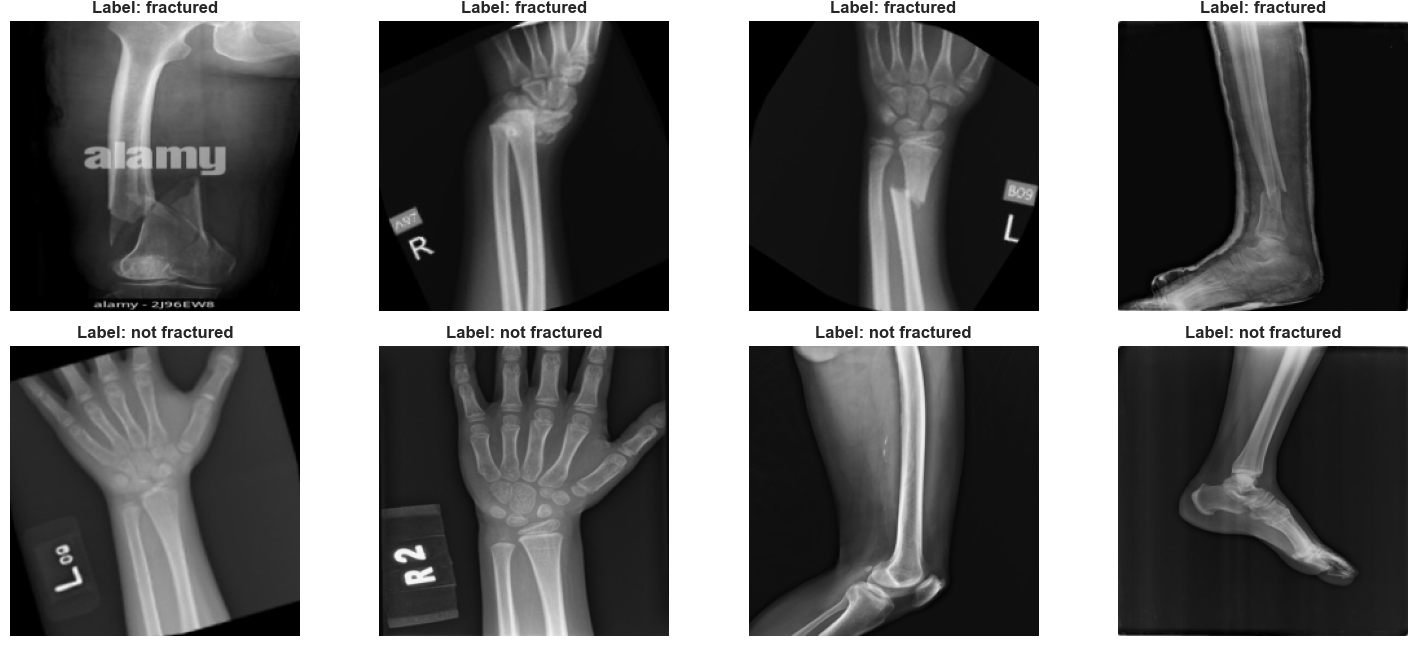
\includegraphics[width=\linewidth]{figures/v1_xray_samples.png}
{\scriptsize\color{ink2} Test X-rays: top row fractured, bottom row not fractured.}
\end{column}
\end{columns}
\end{frame}

% ================================================================ 3
\section{Data}
\begin{frame}{Dataset: Bone Fracture Multi-Region X-ray (Kaggle)}
\begin{columns}[T]
\begin{column}{0.36\textwidth}
\small
\begin{tabular}{@{}lr@{}}
\toprule
split & images \\ \midrule
train & \NTrain \\
val & \NVal \\
test & \NTest \\ \bottomrule
\end{tabular}

\medskip
\begin{itemize}\small
  \item grey X-rays of all body regions, very different sizes
  \item loaded in \textbf{grey}, 224$\times$224
  \item \textbf{train}: CV + final training; \textbf{val}: picks the final epoch; \textbf{test}: used once
  \item augmentation: flip, $\pm$10° rotation, shift, zoom, brightness, contrast
\end{itemize}
\end{column}
\begin{column}{0.62\textwidth}
\resultfig{dataset_overview}
\end{column}
\end{columns}
\end{frame}

% ================================================================ 4
\begin{frame}{Studying the data: the same X-ray appears several times}
\begin{columns}[T]
\begin{column}{0.4\textwidth}
\small
Many images are rotated / flipped / re-cropped copies of one radiograph.
We match 32$\times$32 thumbnails (cosine $\ge 0.97$, 8 flips/rotations):
\begin{itemize}
  \item \DupTrain{} train images (\DupTrainPct\%) have a copy in train (\DupGroups{} groups)
  \item \DupTest{} test images (\DupTestPct\%) have a copy in train
\end{itemize}
\textbf{Consequences}
\begin{itemize}
  \item \alert{grouped} k-fold: copies never cross folds
  \item we also report accuracy on \alert{clean} test images (no copy in train)
\end{itemize}
{\scriptsize\color{ink2} Copies rotated by other angles are missed: counts are a lower bound.}
\end{column}
\begin{column}{0.58\textwidth}
\resultfig{duplicates_train}\\[2pt]
\resulttable[0.8\linewidth]{duplicates}
\end{column}
\end{columns}
\end{frame}

% ================================================================ 5
\section{Models}
\begin{frame}{Three feature extractors, one identical classifier}
\centering
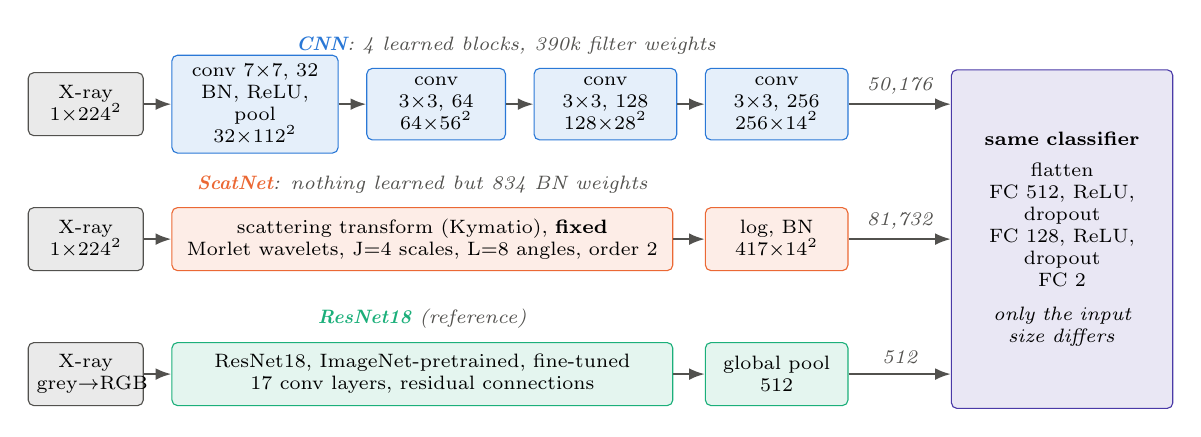
\begin{tikzpicture}[node distance=2.5mm and 3.5mm]
  % CNN row (widths chosen so that the three rows end at the same x)
  \node[blk=ink2, text width=1.25cm] (x1) {X-ray\\1$\times$224$^2$};
  \node[blk=cnn, right=of x1, text width=1.9cm] (c1) {conv 7$\times$7, 32\\BN, ReLU, pool\\32$\times$112$^2$};
  \node[blk=cnn, right=of c1, text width=1.55cm] (c2) {conv 3$\times$3, 64\\64$\times$56$^2$};
  \node[blk=cnn, right=of c2, text width=1.6cm] (c3) {conv 3$\times$3, 128\\128$\times$28$^2$};
  \node[blk=cnn, right=of c3, text width=1.6cm] (c4) {conv 3$\times$3, 256\\256$\times$14$^2$};
  \node[lbl, above=0.5mm of c2.north east] {\textcolor{cnn}{\textbf{CNN}}: 4 learned blocks, 390k filter weights};
  % ScatNet row
  \node[blk=ink2, below=9mm of x1, text width=1.25cm] (x2) {X-ray\\1$\times$224$^2$};
  \node[blk=scat, text width=1.6cm, anchor=east] (s2) at (c4.east |- x2) {log, BN\\417$\times$14$^2$};
  \node[blk=scat, right=of x2, text width=6.15cm] (s1) {scattering transform (Kymatio), \textbf{fixed}\\ Morlet wavelets, J=4 scales, L=8 angles, order 2};
  \node[lbl, above=0.5mm of s1.north] {\textcolor{scat}{\textbf{ScatNet}}: nothing learned but 834 BN weights};
  % ResNet row
  \node[blk=ink2, below=9mm of x2, text width=1.25cm] (x3) {X-ray\\grey$\to$RGB};
  \node[blk=res, text width=1.6cm, anchor=east] (r2) at (c4.east |- x3) {global pool\\512};
  \node[blk=res, right=of x3, text width=6.15cm] (r1) {ResNet18, ImageNet-pretrained, fine-tuned\\ 17 conv layers, residual connections};
  \node[lbl, above=0.5mm of r1.north] {\textcolor{res}{\textbf{ResNet18}} (reference)};
  % classifier
  \node[blk=head, anchor=west, text width=2.6cm, minimum height=4.3cm] (h) at ([xshift=13mm]s2.east) {\textbf{same classifier}\\[3pt]
     flatten\\ FC 512, ReLU, dropout\\ FC 128, ReLU, dropout\\ FC 2\\[4pt] \textit{only the input size differs}};
  \foreach \a/\b in {x1/c1,c1/c2,c2/c3,c3/c4,x2/s1,s1/s2,x3/r1,r1/r2} \draw[arr] (\a) -- (\b);
  \draw[arr] (c4.east) -- node[lbl, above]{50{,}176} (c4.east -| h.west);
  \draw[arr] (s2.east) -- node[lbl, above]{81{,}732} (s2.east -| h.west);
  \draw[arr] (r2.east) -- node[lbl, above]{512} (r2.east -| h.west);
\end{tikzpicture}

\medskip
\small CNN and ScatNet both end on a \textbf{14$\times$14 grid} (4 poolings $\leftrightarrow$ averaging at scale $2^J=16$ px).
Parameters: CNN \ParamsCNN{} \textbullet{} ScatNet \ParamsScat{} (all in the classifier) \textbullet{} ResNet18 \ParamsRes.
\end{frame}

% ================================================================ 6
\begin{frame}{ScatNet: a CNN whose filters are wavelets fixed in advance}
\begin{columns}[T]
\begin{column}{0.45\textwidth}
\small
Morlet wavelets $\psi_{j,\theta}$ (scale $2^j$, angle $\theta$), low-pass $\phi_J$:
\begin{align*}
S_0 x &= x \star \phi_J\\
S_1 x &= |x \star \psi_{j_1,\theta_1}| \star \phi_J\\
S_2 x &= \big||x \star \psi_{j_1,\theta_1}| \star \psi_{j_2,\theta_2}\big| \star \phi_J,\ j_2>j_1
\end{align*}
$1 + JL + L^2\tfrac{J(J-1)}{2} = 1+32+384 = \mathbf{417}$ maps of $\tfrac{224}{2^4}=14^2$.
\begin{itemize}
  \item modulus = non-linearity, averaging = pooling
  \item invariant to shifts $< 2^J$, stable to small deformations
  \item \alert{nothing to learn} (and nothing adapts to fractures)
\end{itemize}
\end{column}
\begin{column}{0.53\textwidth}
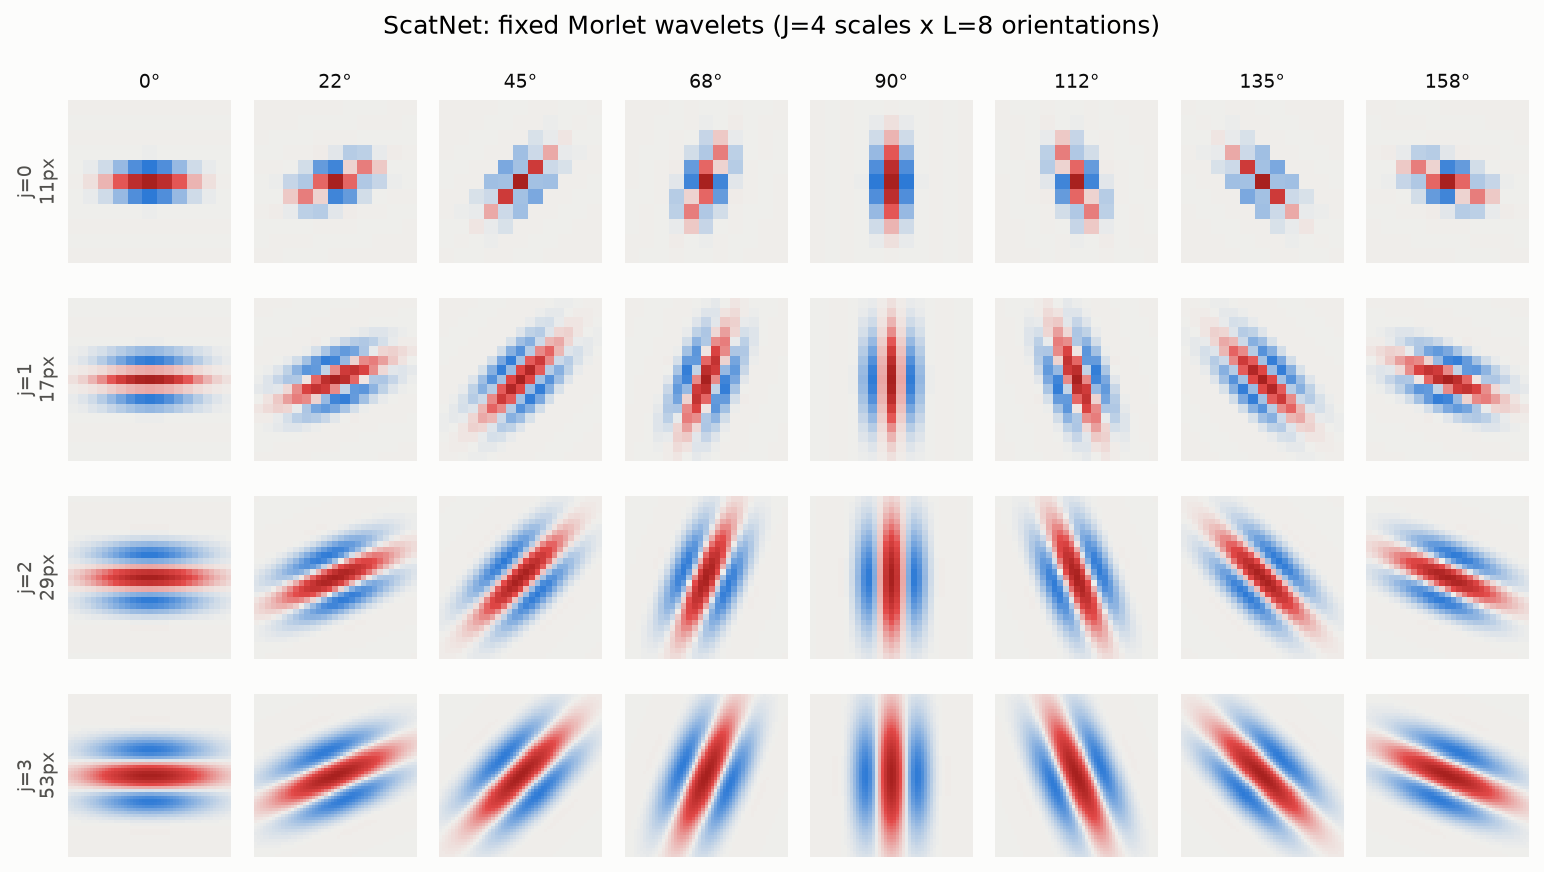
\includegraphics[width=\linewidth]{figures/morlet_wavelets.png}
\end{column}
\end{columns}
\end{frame}

% ================================================================ 7
\begin{frame}{Training and evaluation protocol}
\centering
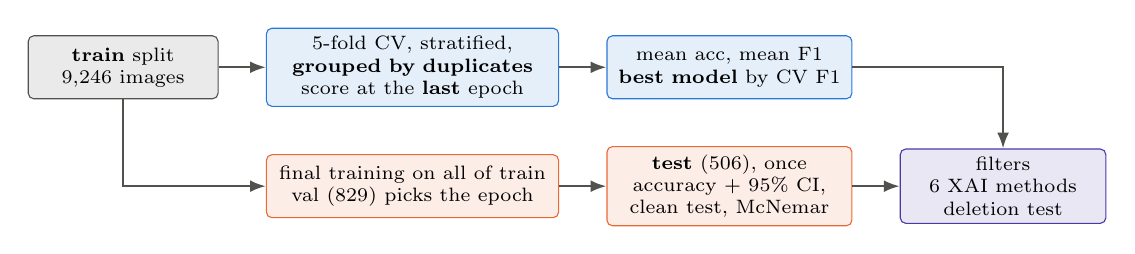
\begin{tikzpicture}[node distance=4mm and 6mm]
  \node[blk=ink2, text width=2.2cm] (tr) {\textbf{train} split\\\NTrain{} images};
  \node[blk=cnn, right=of tr, text width=3.5cm] (cv) {\KFolds-fold CV, stratified,\\\textbf{grouped by duplicates}\\score at the \textbf{last} epoch};
  \node[blk=cnn, right=of cv, text width=2.9cm] (sel) {mean acc, mean F1\\\textbf{best model} by CV \SelectBy};
  \node[blk=scat, below=6mm of cv, text width=3.5cm] (fin) {final training on all of train\\val (\NVal) picks the epoch};
  \node[blk=scat, right=of fin, text width=2.9cm] (te) {\textbf{test} (\NTest), once\\accuracy + 95\% CI, clean test, McNemar};
  \node[blk=head, right=of te, text width=2.4cm] (xai) {filters\\6 XAI methods\\deletion test};
  \draw[arr] (tr) -- (cv); \draw[arr] (cv) -- (sel);
  \draw[arr] (tr) |- (fin); \draw[arr] (fin) -- (te); \draw[arr] (te) -- (xai); \draw[arr] (sel) -| (xai);
\end{tikzpicture}

\bigskip
\begin{columns}[T]
\begin{column}{0.48\textwidth}\small
\begin{itemize}
  \item AdamW, weight decay $10^{-4}$, cosine schedule, \Epochs{} epochs, batch 32
  \item lr $10^{-3}$ (CNN, ScatNet), $10^{-4}$ (ResNet18 fine-tuning)
  \item cross-entropy; F1/recall for the \alert{fractured} class
\end{itemize}
\end{column}
\begin{column}{0.48\textwidth}\small
\begin{itemize}
  \item nothing is selected on a validation fold $\Rightarrow$ CV is not optimistic
  \item the best model is chosen \emph{without} the test set
  \item one command: \texttt{./run.sh push} (Kaggle GPU)
\end{itemize}
\end{column}
\end{columns}
\end{frame}

% ================================================================ 8
\section{Results}
\begin{frame}{Cross-validation on the training set (mean $\pm$ std over \KFolds{} folds, \%)}
\resulttable[0.82\linewidth]{cv}

\medskip
\centering
\resultfig[height=0.52\textheight]{learning_curves}
\end{frame}

% ================================================================ 9
\begin{frame}{Test set (\NTest{} images, used once)}
\resulttable[0.95\linewidth]{test}

\medskip
\begin{columns}[T]
\begin{column}{0.64\textwidth}
\resultfig{confusion_matrices}
\end{column}
\begin{column}{0.34\textwidth}
\resultfig{roc}
\end{column}
\end{columns}
\end{frame}

% ================================================================ 10
\begin{frame}{Which model is best, and why}
\begin{columns}[T]
\begin{column}{0.5\textwidth}
\resultfig{model_comparison}

\small McNemar (same test images): CNN vs ScatNet $p=\McNemarCNNvsScat$,
CNN vs ResNet18 $p=\McNemarCNNvsRes$, ScatNet vs ResNet18 $p=\McNemarScatvsRes$.
\end{column}
\begin{column}{0.48\textwidth}
\small
\textbf{Best by CV \SelectBy: \alert{\BestModel}} \\
test accuracy CNN \TestAccCNN\%, ScatNet \TestAccScat\%, ResNet18 \TestAccRes\% (target $\ge$75\%)

\medskip
\begin{itemize}
  \item \textcolor{scat}{\textbf{ScatNet}}: fixed, generic edge/texture energy at 4 scales $\times$ 8 angles; stable, but cannot adapt to thin, irregular fracture lines; its 42M weights all sit in the classifier
  \item \textcolor{cnn}{\textbf{CNN}}: filters and a hierarchy learned \emph{for} X-rays, from only 9k images
  \item \textcolor{res}{\textbf{ResNet18}}: the same learned hierarchy, deeper, with residual connections and \emph{pre-trained} on 1.2M images $\Rightarrow$ better features from little data, fewest parameters
\end{itemize}
\end{column}
\end{columns}
\end{frame}

% ================================================================ 11
\begin{frame}{Filters: learned (CNN) vs fixed (ScatNet)}
\begin{columns}[T]
\begin{column}{0.5\textwidth}
\resultfig{filters_cnn}
\small
\begin{itemize}
  \item CNN: 32 filters 7$\times$7 learned with augmentation: oriented edges, blobs, contrast detectors
  \item ScatNet: Morlet wavelets, every scale and angle, whether useful or not
\end{itemize}
\end{column}
\begin{column}{0.48\textwidth}
\resultfig{frequency_coverage}
{\scriptsize\color{ink2} Power spectrum of the first layer: wavelets tile the frequency plane uniformly, the CNN concentrates where the X-rays need it.}
\end{column}
\end{columns}
\end{frame}

% ================================================================ 12
\section{Explainability}
\begin{frame}{Six XAI methods, and where they cannot be used}
\centering\small
\begin{tabular}{@{}llp{6.4cm}cc@{}}
\toprule
family & method & idea & CNN & ScatNet \\ \midrule
gradient & Saliency & $|\partial f_c/\partial x|$ & \yes & \yes \\
gradient & Integrated Gradients & $(x-x_0)\int_0^1 \partial_x f_c(x_0+\alpha(x-x_0))\,d\alpha$, $x_0$ = black & \yes & \yes \\
modified gradient & Guided Backprop & only positive signals flow back through the ReLUs & \yes & \half{} partly \\
class activation & Grad-CAM & last conv maps weighted by their mean gradient & \yes & \no{} no \\
perturbation & Occlusion & score drop when a 16$\times$16 window turns black & \yes & \yes \\
surrogate & LIME & ridge model on 1000 random on/off 16$\times$16 patches & \yes & \yes \\ \bottomrule
\end{tabular}

\bigskip
\begin{itemize}\small
  \item \textbf{Grad-CAM} needs a \emph{learned} convolutional feature map: ScatNet's maps are fixed wavelet coefficients $\Rightarrow$ not applicable
  \item \textbf{Guided Backprop} modifies the ReLU backward pass: ScatNet's non-linearity is the complex modulus, so only the classifier is ``guided''
  \item gradient- and perturbation-based methods only need $\partial f/\partial x$ or forward passes $\Rightarrow$ any model
\end{itemize}
\end{frame}

% ================================================================ 13
\begin{frame}{XAI on the CNN (2 images per class, true class explained)}
\centering
\resultfig[height=0.84\textheight]{xai_cnn}
\end{frame}

% ================================================================ 14
\begin{frame}{XAI on ScatNet}
\centering
\resultfig[height=0.84\textheight]{xai_scatnet}
\end{frame}

% ================================================================ 15 (only if the best model is ResNet18)
\ifdefstring{\BestModelKey}{resnet18}{%
\begin{frame}{XAI on the best model: ResNet18}
\centering
\resultfig[height=0.84\textheight]{xai_resnet18}
\end{frame}}{}

% ================================================================ 16
\begin{frame}{Our Occlusion (from scratch) vs Captum's}
\begin{columns}[T]
\begin{column}{0.4\textwidth}
\small
\textbf{Algorithm} (Zeiler \& Fergus 2014)
\begin{enumerate}
  \item score $f_c(x)$ of the class
  \item slide a 16$\times$16 black window, stride 8
  \item drop $f_c(x) - f_c(x_{\text{occluded}})$
  \item each pixel: mean drop of the windows covering it
\end{enumerate}
Plain PyTorch, batched (\texttt{src/occlusion\_scratch.py}).

\medskip
\textbf{Result}: max $|$ours $-$ Captum$|$ = \ScratchMaxDiff, Pearson $r \ge$ \ScratchMinCorr{} on every image and model $\Rightarrow$ identical up to float error (also a unit test).
\end{column}
\begin{column}{0.58\textwidth}
\resultfig{occlusion_scratch_vs_captum}
\end{column}
\end{columns}
\end{frame}

% ================================================================ 17
\begin{frame}{Which method gives the best attributions?}
\begin{columns}[T]
\begin{column}{0.58\textwidth}
\resultfig{deletion_curves}
\end{column}
\begin{column}{0.4\textwidth}
\small
\textbf{Deletion test}: black out 16$\times$16 patches, most important first; a faithful map makes the class probability fall fast (lower area = better; \emph{Random} is the bar to beat).

\medskip
\resulttable[0.95\linewidth]{deletion}

\medskip
Most faithful: CNN \BestXAICNN, ScatNet \BestXAIScat.
\end{column}
\end{columns}
\end{frame}

% ================================================================ 18
\begin{frame}{Do the methods agree?}
\centering
\resultfig[height=0.62\textheight]{xai_agreement}

\small Spearman correlation of patch-level maps. Gradient methods agree with each other,
perturbation methods with each other; the two families disagree more $\Rightarrow$ each answers a different question
(local sensitivity vs effect of removing a region).
\end{frame}

% ================================================================ 19
\section{Conclusions}
\begin{frame}{Discussion and conclusions}
\small
\begin{itemize}
  \item \textbf{Models}: all above the 75\% target; \BestModel{} is best by cross-validation and on the test set.
        Learned (and pre-trained) features beat fixed wavelets for thin, irregular fracture lines;
        ScatNet stays competitive with no learned filter at all.
  \item \textbf{Data}: near-duplicate X-rays inflate scores $\Rightarrow$ grouped CV + clean-test accuracy
        (CNN \CleanAccCNN\%, ScatNet \CleanAccScat\%, ResNet18 \CleanAccRes\%).
  \item \textbf{Filters}: CNN filters look like oriented edge/blob detectors, related to but less uniform than Morlet wavelets.
  \item \textbf{XAI}: perturbation methods (Occlusion, LIME) are the most faithful but 10--100$\times$ slower and coarse;
        gradients are sharp but noisy; Integrated Gradients is the best compromise.
        Grad-CAM does not apply to ScatNet; Guided Backprop only partly.
  \item \textbf{Our Occlusion} = Captum's up to floating-point error.
  \item \textbf{Limits}: rotated duplicates not detected; few explained images; one baseline (black) for all methods.
\end{itemize}
\end{frame}

% ================================================================ backup
\appendix
\begin{frame}{Backup: the previous iteration and what we changed}
\begin{columns}[T]
\begin{column}{0.5\textwidth}
\small
First version (team notebook, 10 epochs, RGB input):
\begin{tabular}{@{}lrr@{}}
\toprule
model & CV acc. & test acc. \\ \midrule
CNN & 97.4 & 92.9 \\
ResNet18 & 98.3 & 94.7 \\
ScatNet & 96.7 & 90.5 \\ \bottomrule
\end{tabular}

\medskip
\textbf{Fixed since}
\begin{itemize}
  \item CNN and ScatNet had \emph{different} classifiers (exam!)
  \item CV folds mixed copies of one X-ray; fold score taken at the best epoch $\Rightarrow$ 4--6 pt gap CV/test
  \item grey baseline for Occlusion (right): highlights the black background
  \item grey images fed as 3 identical channels
\end{itemize}
\end{column}
\begin{column}{0.48\textwidth}
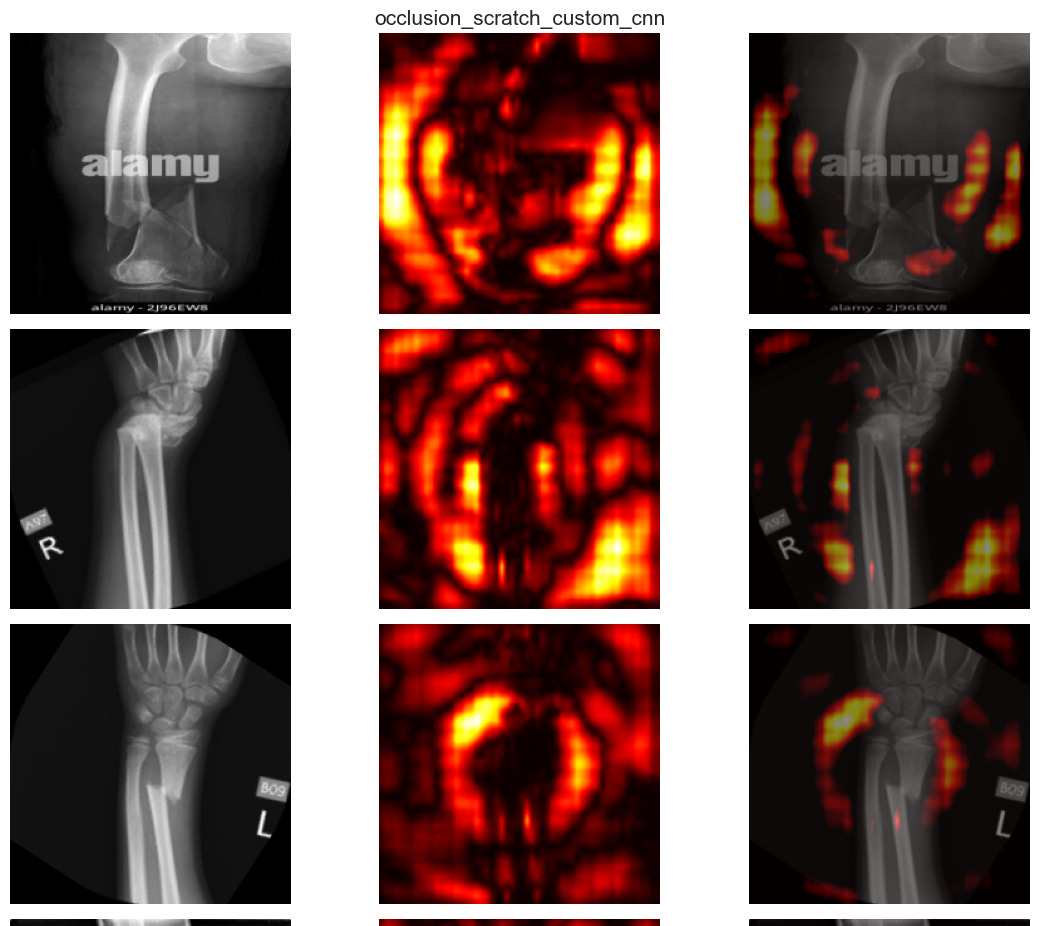
\includegraphics[width=\linewidth]{figures/v1_occlusion_grey_baseline.png}
{\scriptsize\color{ink2} v1 Occlusion with a grey baseline: the evidence sits on the background edges.}
\end{column}
\end{columns}
\end{frame}

\begin{frame}{Backup: reproducibility and tests}
\small
\begin{itemize}
  \item \texttt{notebooks/main.ipynb}: settings + calls to \texttt{src/} (data, models, training, xai, plots, report)
  \item Kaggle: \texttt{./run.sh push [--quick]} $\to$ \texttt{status} $\to$ \texttt{get} $\to$ \texttt{slides}; dataset attached through \texttt{kernel-metadata.json}
  \item \texttt{pytest}: data loading and caching, duplicate detection (planted flips/rotations/leaks), identical classifiers,
        every XAI method on every model, Occlusion scratch = Captum, Integrated Gradients completeness,
        deletion test ranks the right map first, grouped folds never split a group, a model overfits 16 images,
        the whole notebook on synthetic X-rays
  \item seeds fixed; every number in these slides is read from \texttt{results/summary.json}
\end{itemize}
\end{frame}

\end{document}
